\par
Zur Erläuterung dieser Aufzeichnungen bemerken wir folgendes.

Die Ungleichungen [III], [IV] stellen, wenn man \(\alpha=x+yi\) setzt, die
Aussengebiete der beiden Kreise dar, die um die Punkte \(\frac i2\) bezw. \(-\frac i2\) der
lateralen Achse mit dem Radius \(\frac12\) beschrieben sind. Die Ungleichung [I]
bezieht sich offenbar auf eine etwas andere Anordnung der Figur, sie müsste
lauten \(-1<y<1\); die Ungleichung [II] gibt das Aussengebiet des Kreises,
dessen Mittelpunkt im Punkte \(\frac i4\) liegt und dessen Radius gleich \(\frac14\) ist. Die
Formeln auf Seite 8 der Scheda geben das Verhalten der Funktion \((\alpha)=p(\alpha)\)
(wo also \(\alpha\) an Stelle des sonst angewandten \(t\) steht) einmal (Formel 1)) für
die eine Fundamentalsubstitution \(t+2i\) der Hauptkongruenzgruppe zweiter
Stufe, dann aber (Formeln 2), 3)) für die beiden Fundamentalsubstitutionen
\(t+i,\ \frac1t\) der Gruppe (13); diese letzteren Formeln stimmen also mit den des
Art. 6 der Notiz 3), d. h. mit den beiden ersten Gleichungen unserer Formelsysteme (16),
(17) überein\footnote{In der Tat ist \(2(4\alpha)-(\alpha)=q(\alpha)\), vergl. die Fussnote \textsuperscript{131a)}.}. — Auf die funktionentheoretische Bedeutung der Figur 1 geht \textsc{Gauss} hier
nicht ein, wir müssen darum gleich die Aufzeichnung 7) mit heranziehen (Werke III,
S. 477, Art. 12), in der das Funktionentheoretische vollständig gegeben ist. Wir finden
daselbst einen Ausschnitt der Figur 1 (siehe die Figur 2), nämlich den Bereich, oder wie \textsc{Gauss}
sagt »Raum«, der arithmetisch dadurch charakterisiert ist, dass in ihm »der
imaginäre Teil von \(t\) und \(\frac1t\) zwischen \(-i\) und \(+i\) liegt«.
\begin{center}
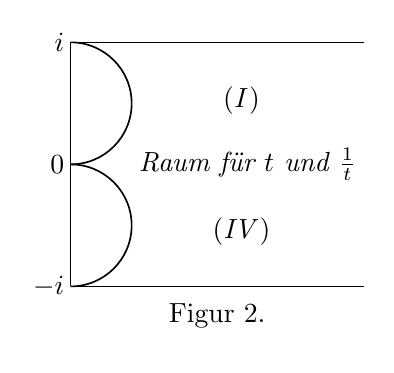
\begin{tikzpicture}[x=1.55cm,y=1.55cm,line width=.6pt]
\draw (0,-1)--(0,1)--(2.4,1);
\draw (0,-1)--(2.4,-1);
\draw (0,1) arc[start angle=90,end angle=-90,radius=.5];
\draw (0,0) arc[start angle=90,end angle=-90,radius=.5];
\node[left,inner sep=2pt] at(0,1){\(i\)};
\node[left,inner sep=2pt] at(0,0){\(0\)};
\node[left,inner sep=2pt] at(0,-1){\(-i\)};
\node at(1.4,.52){\(\mathit{(I)}\)};
\node at(1.4,-.55){\(\mathit{(IV)}\)};
\node at(1.45,0){\textit{Raum für \(t\) und \(\frac1t\)}};
\node[below,inner sep=6pt] at(1.2,-1){Figur 2.};
\end{tikzpicture}
\end{center}
\noindent In diesem Bereiche\par
\clearpage\SourceLeaf{189}\ArithmeticHead{104}{L}{L. SCHLESINGER, ÜBER GAUSS’ FUNKTIONENTHEORETISCHE ARBEITEN.}
\noindent \(F_2\) ist nun — so heisst es weiter — »der reelle Teil von \(q(t)^2/p(t)^2\)«, also von
\(k'\), »positiv«, was »geometrisch zu beweisen« sei. In der Tat zeigt die Betrachtung
von \(k'\) auf der Begrenzung des Bereichs \(F_2\) und auf der positiven
reellen Achse der \(t\)-Ebene, dass der oberen Hälfte (I) von \(F_2\) der
erste, der unteren Hälfte (IV) von \(F_2\) der vierte Quadrant der \(k'\)-Ebene
gegenseitig eindeutig entspricht\footnote{Vergl. \textsc{Geppert} a. a. O. \textsuperscript{83)}, S. 135, 136, Math. Annalen 99, 1928, S. 167, 168.}. Dem zweiten und dritten Quadranten
der \(k'\)-Ebene entsprechen dann, nach dem Symmetrieprinzip, die Spiegelbilder
jener Bereichhälften (I), (IV) in bezug auf die begrenzenden Kreise,
also die in der Figur 1 sichtbaren Kreisbogendreiecke (II), (III), so dass in
dem Kreisbogensechseck mit den Ecken \(+\infty,i,\frac12i,0,-\frac12i,-i\) die Funktion
\(k'\) jeden Wert einmal und nur einmal annimmt. \textsc{Gauss'} Angabe (Werke III,
S. 478), dass »die Gleichung \(k'=q(t)^2/p(t)^2\) in dem« in der Figur 3 veranschaulichten »Raume, immer
eine und nur eine Auflösung hat« ist demnach dahin einzuschränken, dass dies nur für die Werte
von \(k'\) gilt, deren absoluter Betrag nicht grösser ist als 1\footnote{Vergl. \textsc{Fricke}, Werke VIII, S. 105.}.
\begin{center}
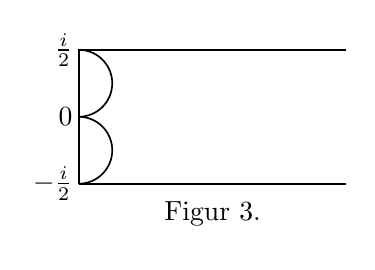
\begin{tikzpicture}[x=1.7cm,y=1.7cm,line width=.6pt]
\draw (0,-.5)--(0,.5)--(2,.5);
\draw (0,-.5)--(2,-.5);
\draw (0,.5) arc[start angle=90,end angle=-90,radius=.25];
\draw (0,0) arc[start angle=90,end angle=-90,radius=.25];
\node[left,inner sep=2pt] at(0,.5){\(\frac i2\)};
\node[left,inner sep=2pt] at(0,0){\(0\)};
\node[left,inner sep=2pt] at(0,-.5){\(-\frac i2\)};
\node[below,inner sep=6pt] at(1,-.5){Figur 3.};
\end{tikzpicture}
\end{center}
\noindent Daraus, dass in dem Bereiche \(F_2\) die
Funktion \(k'\) alle Werte des ersten und vierten Quadranten einmal und nur
einmal annimmt, folgt zunächst, wie \textsc{Gauss} anmerkt, dass, wenn man aus
\[
\mu p(\tfrac12t)^2,\quad\mu q(\tfrac12t)^2
\]
\noindent das »einfachste agM.« bildet\footnote{D. h. dasjenige, wo bei den geometrischen Mitteln \(\sqrt{a_{\nu-1}b_{\nu-1}}\) das Vorzeichen immer so gewählt wird, dass der reelle Teil von \(\frac{\sqrt{a_{\nu-1}b_{\nu-1}}}{a_{\nu-1}}\) positiv ausfällt.}, dieses den Wert \(\mu\) hat, vorausgesetzt, dass \(t\)
in jenem Bereiche gelegen ist. Ferner ergibt sich daraus sofort, dass die
Modulfunktion \(k'^2=q(t)^4/p(t)^4\) in \(F_2\) jeden Wert nur einmal annimmt (natürlich
mit den für die Begrenzung geltenden üblichen Festsetzungen), dass also
\(F_2\) den Fundamentalbereich der Modulfunktion oder der Hauptkongruenzgruppe
zweiter Stufe darstellt\footnote{Die Art wie \textsc{Schering} Werke III, S. 477, 478 die Figuren 2 und 3 wiedergegeben hat, zeigt, dass er ihre Bedeutung nicht erkannt hatte. — Vor der Öffentlichkeit hat wohl zuerst \textsc{Klein} (Mathem. Annalen 21, S. 215 und \textsc{Klein-Fricke}, \textit{Vorlesungen über die Theorie der elliptischen Modulfunktionen} I, 1890, S. 278, Fussnote) diese Bedeutung hervorgehoben. In korrekter Zeichnung sind jene Figuren durch \textsc{Fricke} Werke VIII, S. 105 reproduziert worden.}.
\clearpage\SourceLeaf{190}\ArithmeticHead{105}{R}{Vc. THEORIE DER MODULFUNKTION.}
\HistoricalFoot{X 2 Abh. 2.}{14}
\noindent\hspace*{\parindent}Die Tatsache, dass weder in den Formeln, noch in der Figur 1 der Scheda
An die Bedingung \(x>0\) hervortritt, lässt vermuten, dass \textsc{Gauss} beim Entwerfen
jener Figur \textls[100]{rein zahlentheoretisch} den geometrischen Ort der
Werte \(t=\frac{\pm1+bi}a\) für die reduzierte quadratische Form \((a,b,c)\) (ohne Beschränkung
auf den Wert mit positivem reellen Teil) aufgesucht und \textls[100]{nicht} etwa
\textls[100]{funktionentheoretisch} gedacht hat.\linebreak Dass er aber gleich hinterher die
funktionentheoretische Bedeutung der Figur in Betracht zog, zeigen die Formeln
auf S. 8 der Scheda. Der Umstand, dass \textsc{Gauss} auch den Kreis
\(x^2+y^2=1\) hingezeichnet hat, beweist, dass er nicht nur den Fundamentalbereich
der Hauptkongruenzgruppe zweiter Stufe im Auge hatte, sondern auch
den Fundamentalbereich der Modulgruppe (13) betrachtet hat. Dieser, d. h.
der geometrische Ort der Punkte \(t=\frac{1+bi}a\) für die reduzierte Form \((a,b,c)\)
mit der Determinante \(-1\), ist der Teil der rechten \(t\)-Halbebene, der ausserhalb
des Einheitskreises und zwischen den Geraden \(y=\pm\frac12\) gelegen ist.
Dass die oben definierte Funktion \(f(t)\) in diesem Bereiche \(F\) jeden komplexen
Wert einmal und nur einmal annehmen sollte, hatte \textsc{Gauss}, wie
wir gesehen haben, festgestellt; in der nachgaussischen Literatur tritt dieser
Bereich wohl zuerst bei \textsc{Dedekind} (a. a. O. \textsuperscript{138)}, S. 180) als das \textls[100]{Hauptfeld}
auf. Nach der Anlage der in der Handschrift nur skizzierten Figur 1
scheint es nicht ausgeschlossen, dass \textsc{Gauss} auch die Einlagerung des Fundamentalbereichs
\(F\) der Modulgruppe (13) in den der Hauptkongruenzgruppe
zweiter Stufe \(F_2\) ins Auge gefasst und damit die sechs Fälle der Substitutionen
(13) modulo 2 geometrisch interpretiert hat.

Unzweifelhaft hat \textsc{Gauss} (wie auch \textsc{Fricke}, Werke VIII, S. 103, 104 hervorhebt)
bei diesen Betrachtungen die Bedeutung der Spiegelung an Kreisen
für die Zusammensetzung der Fundamentalsubstitutionen \(t+i,\ \frac1t\) erkannt und bei
der geometrischen Darstellung der durch die Substitutionen (13) gegebenen
\(t'\)-Werte zur Anwendung gebracht\footnote{Man vergl. auch die Nachlassnotizen Werke VIII, S. 354, 355, die von den Beziehungen zwischen lineargebrochenen Substitutionen und den Drehungen einer Kugel handeln.}, auch gibt eine aus dem Nachlass stammende
Zeichnung, die Werke VIII, S. 104 wiedergegeben ist, (darstellend ein
Netz von Kreisbogendreiecken mit Orthogonalkreis) die Gewissheit, dass ihm\par
\clearpage\SourceLeaf{191}\ArithmeticHead{106}{L}{L. SCHLESINGER, ÜBER GAUSS’ FUNKTIONENTHEORETISCHE ARBEITEN.}
\noindent bekannt war, wie das durch jenes Spiegelungsprinzip aus den Bereichen \(F\)
bezw. \(F_2\) gewonnene Netz die rechte \(t\)-Halbebene überdeckt und die laterale
Achse zur natürlichen Grenze hat.

Das Werke VIII, S. 99—102, abgedruckte Fragment 5) stammt aus dem
1815/1816 benutzten Handbuche 25, Bf, es enthält die Auflösung der Gleichung
\[
\frac{q(t)}{p(t)}=A,
\]
\noindent indem \(A^2=k'\) gesetzt und dann ein Wert von \(t\) durch die Formel (18) bestimmt
wird. Die übrigen, sagt \textsc{Gauss}, sind in der Formel (22) »enthalten«,
was ja durchaus richtig ist, aber diese Formel gibt — wie \textsc{Fricke} a. a. O.
bemerkt — nicht nur diese Werte, sondern auch alle Lösungen der Gleichung
\[
k'^2=\frac{q(t)^4}{p(t)^4}.
\]

Wahrscheinlich war \textsc{Gauss}, abgesehen von der vielleicht erst 1805 gefundenen
geometrischen Repräsentation des Fundamentalbereichs, im Juni 1800
bereits im Besitz der wesentlichsten dieser Eigenschaften der Modulfunktion.
